\documentclass{article}
\usepackage{graphicx} % Required for inserting images
\usepackage{float}
\usepackage[T1]{fontenc}
\usepackage{amsmath}
\usepackage[margin=1in]{geometry}
\usepackage{booktabs}
\usepackage{tabularx}
\usepackage[hidelinks]{hyperref}

\title{Straddles and strangles on the VRP-band book: more P\&L, not less volatility}
\author{Experiment report \textperiodcentered{} L/S Gamma Desk, QUANTT}
\date{2026-11-13}

\begin{document}

\maketitle

\textbf{Question:} on the VRP-band rules, does trading an ATM straddle for long gamma and a 20-delta strangle for short gamma (1 contract per leg) make the book's daily net P\&L less volatile than the single ATM call or put it trades now, without a deeper drawdown, a worse tail, or more than \$1,000 less net P\&L?

\textbf{Method:}

\begin{itemize}

\item Pre-registered backtest: the hypothesis card and pass bar were committed before any run (commit 7d70155).

\item The VRP-band research baseline (\texttt{configs/\allowbreak{}paper.\allowbreak{}toml} + \texttt{configs/\allowbreak{}backtest.\allowbreak{}toml}) is replayed on R2 replay snapshots v1 (config\_hash b040760187f0) over the development window, 2014-06-02 to 2024-12-31. The out-of-sample window (2025-01-01 to 2026-07-10) was not used.

\item Variants:

\begin{itemize}

\item \texttt{both} (primary): straddle on long signals, 20-delta strangle on short signals.

\item \texttt{straddle\_\allowbreak{}only}: straddle on long signals; short signals keep the ATM put.

\item \texttt{strangle\_\allowbreak{}only}: strangle on short signals; long signals keep the ATM call.

\end{itemize}

Comparison: the registered baseline run matching the current config, at the same spread multiple.

\item Every variant was run at 1x and 2x spreads. Costs:

\begin{itemize}

\item \$0.65 per contract and \$0.005 per share, with a \$1 minimum per order;

\item a structure's two legs are charged as one order;

\item each leg fills at its own quoted half-spread.

\end{itemize}

Signals, exits and hedges run once a day at 10:15 ET.

\item A structure exits as one position: the \texttt{paper.\allowbreak{}toml} exit rules are applied to the legs' combined P\&L (options plus hedge shares) and combined premium, and both legs are sent to close together. One exception is in the caveats.

\end{itemize}

\section{Result vs the pass bar}

Every check had to hold at 1x and 2x. ``Vol'' is the standard deviation of daily net P\&L in USD, flat days included. ES is the mean of the worst 5\% of daily net P\&L. Everything is at one contract per leg.

\begin{center}\small
\begin{tabularx}{\linewidth}{>{\raggedright\arraybackslash}X l l l l l}
\toprule
\textbf{Check (\texttt{both} vs baseline)} & \textbf{1x value} & \textbf{1x bar} & \textbf{2x value} & \textbf{2x bar} & \textbf{Result} \\
\midrule
Vol, full window, lower & \$54.37 & \$35.64 & \$54.75 & \$37.28 & fail \\
Vol, 2014-2019, lower & \$25.80 & \$16.31 & \$26.51 & \$17.84 & fail \\
Vol, 2020-2024, lower & \$74.30 & \$48.94 & \$74.61 & \$50.88 & fail \\
Max drawdown, lower & \$3,848 & \$3,027 & \$4,405 & \$4,258 & fail \\
ES 5\% magnitude within 1.10x & \ensuremath{-}\$137.8 & \ensuremath{-}\$106.1 & \ensuremath{-}\$142.3 & \ensuremath{-}\$115.0 & fail \\
Net P\&L \ensuremath{\geq} baseline \ensuremath{-} \$1,000 & \ensuremath{-}\$318 & \ensuremath{-}\$3,060 & \ensuremath{-}\$1,855 & \ensuremath{-}\$5,122 & pass \\
Event floor: 20 straddles and 20 strangles (1x) & 30 and 102 &  &  &  & met \\
\bottomrule
\end{tabularx}
\end{center}

\textbf{Verdict: failed.} The two-leg book is more volatile than the single-leg book in every period and at both spread levels, and its drawdown and tail are worse. It lost less money: \ensuremath{-}\$318 against \ensuremath{-}\$2,060 at 1x, and all of that gain came from the strangle. No variant made money at 2x except \texttt{strangle\_\allowbreak{}only} (+\$302).

\subsection{Full-window numbers (not part of the bar)}

\begin{center}\small
\begin{tabularx}{\linewidth}{>{\raggedright\arraybackslash}X l l >{\raggedright\arraybackslash}X >{\raggedright\arraybackslash}X l >{\raggedright\arraybackslash}X}
\toprule
\textbf{} & \textbf{baseline 1x} & \textbf{both 1x} & \textbf{straddle\_only 1x} & \textbf{strangle\_only 1x} & \textbf{both 2x} & \textbf{strangle\_only 2x} \\
\midrule
Net P\&L & \ensuremath{-}\$2,060 & \ensuremath{-}\$318 & \ensuremath{-}\$3,783 & +\$1,398 & \ensuremath{-}\$1,855 & +\$302 \\
Vol (daily std) & \$35.64 & \$54.37 & \$48.40 & \$43.54 & \$54.75 & \$43.96 \\
Sharpe & \ensuremath{-}0.36 & \ensuremath{-}0.04 & \ensuremath{-}0.48 & 0.20 & \ensuremath{-}0.21 & 0.04 \\
Max drawdown & \$3,027 & \$3,848 & \$4,765 & \$2,435 & \$4,405 & \$2,754 \\
ES 5\% (daily) & \ensuremath{-}\$96.5 & \ensuremath{-}\$137.8 & \ensuremath{-}\$122.6 & \ensuremath{-}\$114.7 & \ensuremath{-}\$142.3 & \ensuremath{-}\$118.0 \\
Structures (long /\allowbreak{} short) & 30 /\allowbreak{} 101 & 30 /\allowbreak{} 102 & 30 /\allowbreak{} 101 & 30 /\allowbreak{} 102 & 30 /\allowbreak{} 102 & 30 /\allowbreak{} 102 \\
Commissions (options /\allowbreak{} hedges) & \$262 /\allowbreak{} \$914 & \$343 /\allowbreak{} \$878 & \$280 /\allowbreak{} \$916 & \$325 /\allowbreak{} \$876 & \$343 /\allowbreak{} \$878 & \$325 /\allowbreak{} \$876 \\
\bottomrule
\end{tabularx}
\end{center}

The registry's \texttt{trades} column counts legs (264 for \texttt{both}), so the table counts structures instead.

\section{Charts}

\begin{figure}[H]\centering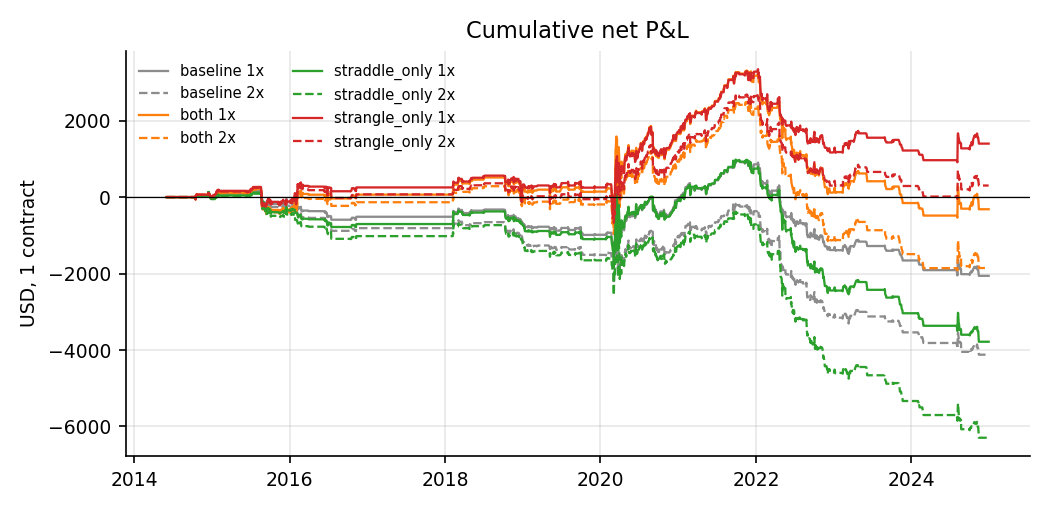
\includegraphics[width=0.92\linewidth]{figures/cum_pnl.png}\caption{Cumulative net P\&L, 1x solid and 2x dashed; baseline grey}\end{figure}

The strangle variants pull ahead in 2020 and 2021 and give back part of it in 2022. \texttt{straddle\_\allowbreak{}only} tracks below the baseline from 2022 on.

\begin{figure}[H]\centering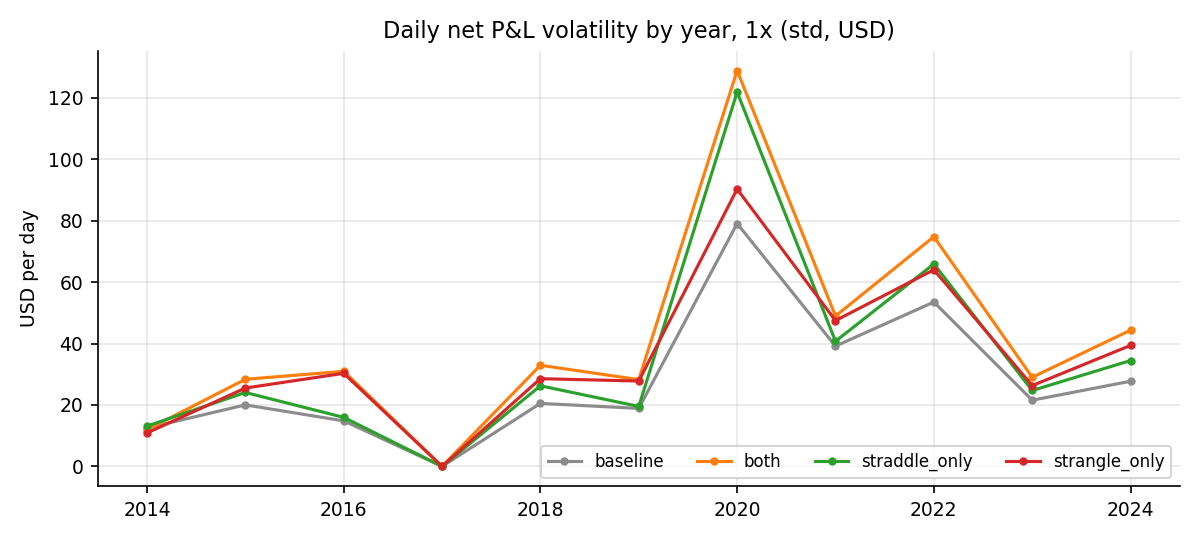
\includegraphics[width=0.92\linewidth]{figures/vol_by_year.png}\caption{Daily net P\&L volatility by year, 1x}\end{figure}

\texttt{both} is above the baseline in every full year that traded (2017 had no positions; 2014 is a half year, \$11.9 against \$12.5), and most of all in 2020. Each half adds volatility on its own.

\begin{figure}[H]\centering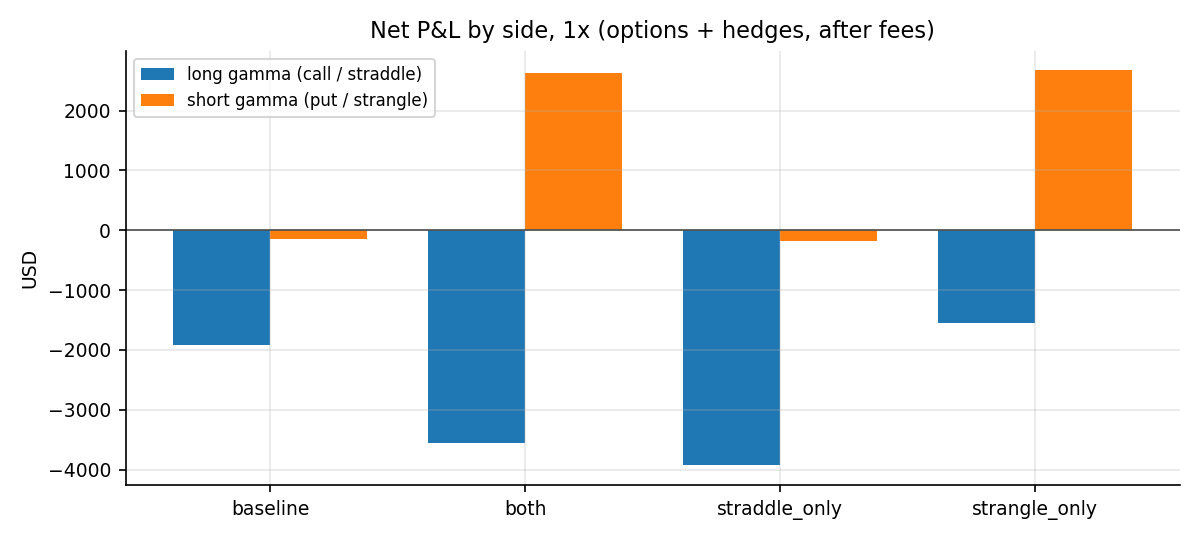
\includegraphics[width=0.92\linewidth]{figures/by_side.png}\caption{Net P\&L by side, 1x}\end{figure}

The long side loses more with a straddle (\ensuremath{-}\$3,555 in \texttt{both} against \ensuremath{-}\$1,913 for the call). The short side turns from \ensuremath{-}\$148 with the ATM put to +\$2,632 with the strangle.

\begin{figure}[H]\centering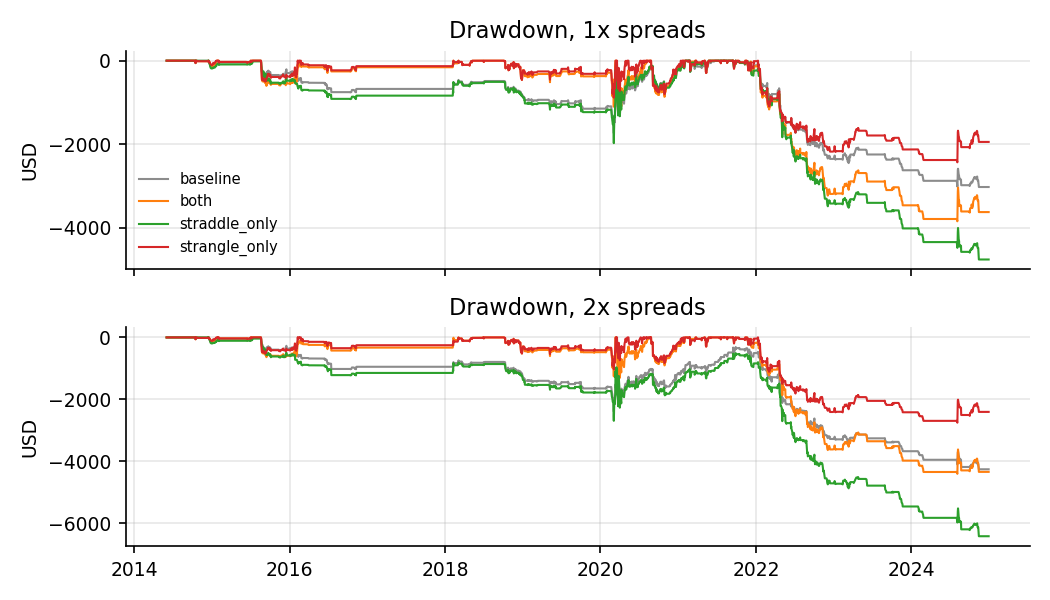
\includegraphics[width=0.92\linewidth]{figures/drawdown.png}\caption{Drawdown at 1x and 2x spreads}\end{figure}

Most of the drawdown in every variant is 2022 and after. \texttt{strangle\_\allowbreak{}only} has the shallowest drawdown at both multiples, and \texttt{straddle\_\allowbreak{}only} the deepest.

\begin{figure}[H]\centering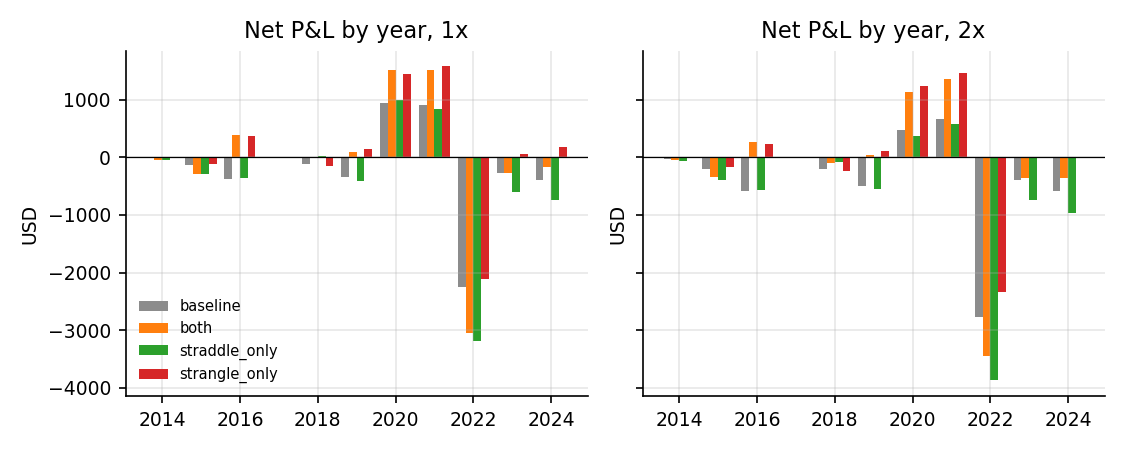
\includegraphics[width=0.92\linewidth]{figures/yearly.png}\caption{Net P\&L by year}\end{figure}

2022 is the worst year for every variant. The straddle makes 2022 worse (\texttt{both} \ensuremath{-}\$3,056 against \ensuremath{-}\$2,242 for the baseline at 1x, by day).

\begin{figure}[H]\centering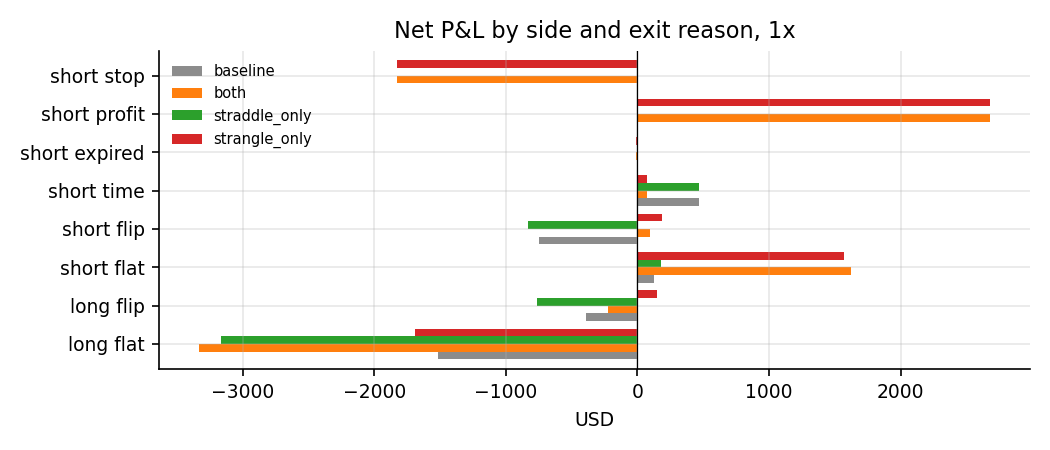
\includegraphics[width=0.92\linewidth]{figures/by_reason.png}\caption{Net P\&L by side and exit reason, 1x}\end{figure}

Bars are per leg, by each leg's own exit reason. Counted per structure, strangles hit the 50\% profit take 9 times (+\$2,670) and the 1x-credit stop 4 times (\ensuremath{-}\$1,827). The ATM put hit neither in 101 round trips; it closed on flat, flip and time.

\begin{figure}[H]\centering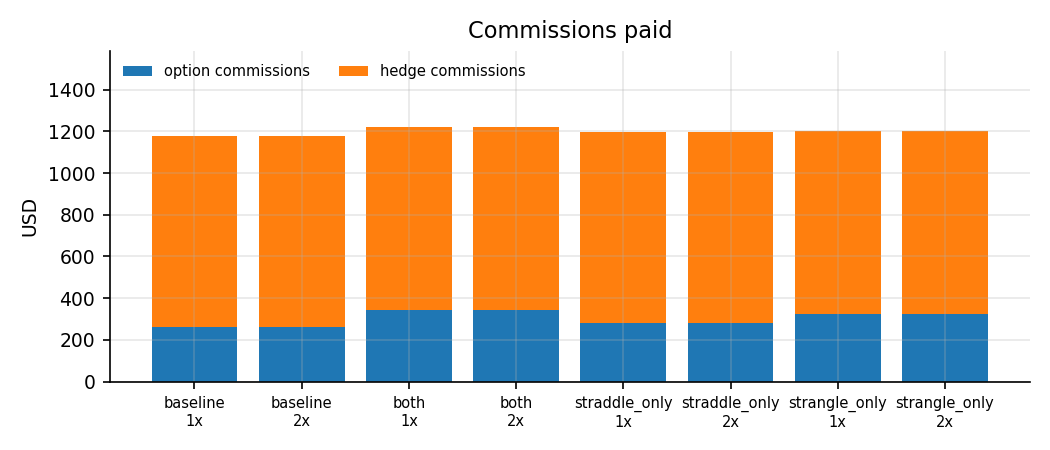
\includegraphics[width=0.92\linewidth]{figures/fees.png}\caption{Commissions paid}\end{figure}

The second leg adds \$81 of option commission over the window in \texttt{both} at 1x. Hedge commission falls slightly with the strangle (\$876 against \$914), which opens close to delta-neutral. \texttt{straddle\_\allowbreak{}only} pays about the same (\$916).

\section{Analysis}

\textbf{The volatility result is mechanical.} At one contract per leg, both structures carry more gamma and vega than the single leg they replace. This was measured from the entry snapshot for every structure at 1x:

\begin{itemize}

\item A straddle averages 2.0x the gamma and 2.0x the vega of the ATM call. It also costs about 2x the premium.

\item A 20-delta strangle averages 1.4x the gamma and 1.4x the vega of the ATM put, for about 60\% of the put's credit.

\end{itemize}

More vega means larger daily P\&L swings, whatever the delta hedge does. Vol rose in every full year that traded (2015-2024, except 2017 with no positions) for \texttt{straddle\_\allowbreak{}only} and \texttt{strangle\_\allowbreak{}only} alike, so neither half delivers the hypothesis. The worst day in all four books is 2020-03-20. The straddle made that day worse (\ensuremath{-}\$786 against \ensuremath{-}\$468); the strangle did not change it.

\textbf{The P\&L gain is the strangle's exit rules, not its lower gamma.} The baseline's ATM put never reached the 50\% profit take or the 1x-credit stop in 101 round trips. A strangle's credit is smaller, and both legs decay while SPY stays between the strikes, so the 50\% target was reached 9 times. Those 9 exits made +\$2,670, more than the short side's whole net P\&L (+\$2,632). The 4 stops cost \ensuremath{-}\$1,827.

The result is concentrated:

\begin{itemize}

\item The 5 best strangles made \$1,933 of the short side's \$2,632.

\item Without them, the short side is +\$699.

\item By year, most of the gain is 2020 and 2021 (+\$2,324 of the \$2,632, by exit date).

\end{itemize}

\textbf{The straddle loses more for the same reason the call does.} Long signals fire when IV is below the RV forecast. The 2026-10-16 short-only card found that the long calls lose money on this window anyway. A straddle doubles that bet's size: 30 straddles lost \ensuremath{-}\$3,555 against \ensuremath{-}\$1,913 for 30 calls. The loss is concentrated in straddles closed in 2022 (\ensuremath{-}\$2,011) and 2023-2024.

\textbf{Path dependence:}

\begin{itemize}

\item All 30 long entries fall on the same dates in every variant.

\item Short entries differ: 93 of the baseline's 101 short entry dates are shared with \texttt{both}, because profit takes and stops end positions earlier and the next entry moves.

\item The long side of \texttt{strangle\_\allowbreak{}only} (\ensuremath{-}\$1,545) differs from the baseline's (\ensuremath{-}\$1,913) with the same calls, because exits and re-entries around the strangles change when positions end.

\end{itemize}

Differences of a few hundred dollars between variants are within that noise.

\section{Verdict}

\textbf{Failed, per the pre-registered bar:} volatility, drawdown and the tail are all worse at 1x and 2x, and only the P\&L floor held. As specified (one contract per leg), the two-leg structures add risk rather than remove it. Archive this card.

The most interesting side result is \texttt{strangle\_\allowbreak{}only} (+\$1,398 /\allowbreak{} +\$302). It was reported only and was not judged by this bar. Its edge rests on 9 profit takes and the 2020-2021 years, and it is the only variant positive at 2x. A follow-up would need its own card: for example, a 20-delta strangle against the ATM put on net P\&L and Sharpe, with gamma matched, so that size is not the difference.

\section{Caveats}

\begin{itemize}

\item \textbf{In-sample:} the idea follows the short-only, trend-long-band and lower-delta results on this same window. Only the out-of-sample run can confirm any of it.

\item \textbf{Size:} one contract per leg, so the structures are not risk-matched with the baseline. The volatility comparison mostly measures size.

\item \textbf{Fills:} each leg is filled separately at its own half-spread. A combo order would usually fill better, so the 2x run is the stress test.

\item \textbf{Spread model:} fitted on about two weeks of calm 2026 live quotes.

\item \textbf{Data gaps:} R2 has no month-end weekdays, so about 3.3\% of scheduled times are skipped.

\item \textbf{One split structure:} 1 of 102 strangles (early 2016) closed its legs separately. One leg had no mark and could not be filled for about two weeks, so it stayed open alone until expiry; the book also went unhedged on those 14 days. The effect was about \ensuremath{-}\$11.

\item \textbf{Few events:} 30 straddles, 9 strangle profit takes and 4 strangle stops drive the differences.

\end{itemize}

\section{Trials}

6 trials for this experiment (3 variants \ensuremath{\times} 1x and 2x, one run of \texttt{experiment.\allowbreak{}py}, commit 7d70155), plus the baseline's 4 registered runs. The comparison used the 2026-11-11 baseline pair, the first that matches the current config (it reproduces the original baseline exactly). There were no rebuilds and no \texttt{-\allowbreak{}dirty} rows. The pass bar was not changed.

\end{document}
